\startchapter{Framework}
\label{chapter:framework}

\section{Introduction}
In Chapters~\ref{chapter:idioms} and \ref{chapter:smells}, we identified that Copilot does not perform well in detecting and suggesting language idioms and best practices, 
the scope of capability for \cct{} like Copilot is uncertain. In this chapter, we try to address \textbf{RQ-1} (What are the current boundaries of code completion tools) with a taxonomy of 5 software abstraction levels to help access the current capabilities of Copilot. 

We explain each software abstraction level in the taxonomy and the capabilities required by \cct{} to satisfy the software abstraction level. 
We try to delineate where current \cct{} are currently best able to perform, and where more complex software engineering tasks overwhelm them. We use a sorting routine as an example scenario to show how a \cct{} suggestion looks like at every level of abstraction in our taxonomy.

\subsection{Motivation}
To center our analysis on creating a software abstraction hierarchy, we leverage an analogous concept in the more developed (but still nascent) field of autonomous driving. 
Koopman has adapted the SAE Autonomous Driving safety levels~\cite{sae} to those shown in figure~\ref{fig:koopman_pyramid}. 
The pyramid concept is derived from that of Maslow~\cite{Maslow1943}, such that addressing aspects on the top of the pyramid first require the satisfaction of aspects below. 
For example, before being able to think about system safety (such as what to do in morally ambiguous scenarios), the vehicle must first be able to navigate its environment reliably (``Basic Driving Functionality'').

We think that a similar hierarchy exists in \AISE{}. Before worrying about software architecture issues, that is, satisfying system quality attributes such as performance, \AISE{} tools need to be able to exhibit ``basic programming functionality''. This basic functionality is where most research effort is currently concentrated, such as program synthesis, \cct{}, and automated bug repair.

\begin{figure}[hbt!]
    \centering
    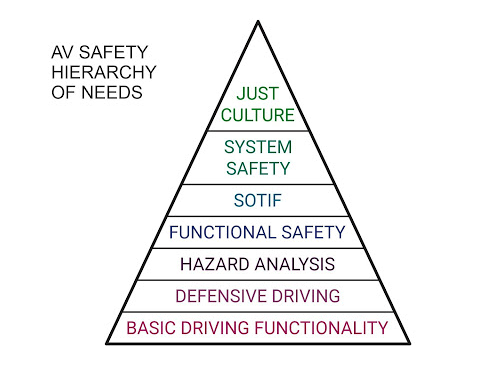
\includegraphics[width=.8\linewidth]{Figures/koopman_pyramid.png}
    \caption{Koopman's Autonomous Vehicle Safety Hierarchy of Needs~\cite{koopman}. SOTIF = safety of the intended function.}
    \label{fig:koopman_pyramid}
\end{figure}

\section{Taxonomy}
\label{taxonomy}
Our taxonomy is a software abstraction hierarchy where ``basic programming functionality'' such as code compilation and syntax checking is the lowest abstraction level,
Software architecture analysis and design are at the highest abstraction level.
As we ascend the levels, just as with Koopman's pyramid in figure \ref{fig:koopman_pyramid}, 
software challenges rely more on human input and become more difficult to automate (e.g., crafting design rules vs. following syntax rules).

Figure~\ref{fig:taxonomy} shows the taxonomy of autonomy levels for \cct{}. The more abstract top levels depend on the resolution of the lower ones. As we move up the hierarchy, we require more human oversight of the AI; as we move down the hierarchy, rules for detecting problems are easier to formulate. Green levels are areas where \cct{} like Copilot works reasonably well, while red levels are challenging for Copilot based on tests shown in Chapter~\ref{chapter:methodology}.

\begin{figure}[hbt!]
    \centering
    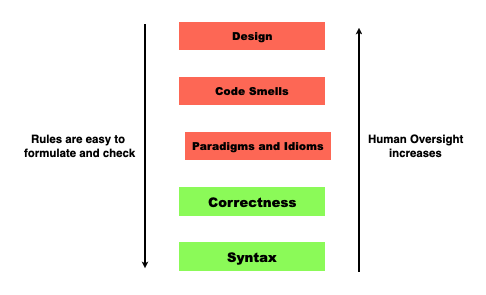
\includegraphics[width=\linewidth]{Figures/taxonomy.png}
    \caption{Hierarchy of software abstractions. Copilot cleared all green levels and struggled in red levels}
    \label{fig:taxonomy}
\end{figure}

Based on our tests with Copilot shown in chapter~\ref{chapter:methodology}, Copilot was able to generate syntactically correct code that solves the given programming task in the coding scenario~(shown in ~\repl{}).
This functionality covers the syntax and the correctness level in our software abstraction hierarchy.
As a result, Copilot stands at the correctness level of our taxonomy. 

The challenges further up the hierarchy are nonetheless more important for software quality attributes (QA)~\cite{Ernst2017} and for a well-engineered software system.
For example, an automated solution suggested by \cct{} to the top level of the taxonomy would be able to follow heuristics to engineer a well-designed software system, which would be easy to modify and scale to sudden changes in use.
\subsection{Syntax}
\label{syntax}
The syntax level is the lowest abstraction level in our taxonomy. This level includes the most basic programming functionality like syntax and code compilations. This level does not require the \cct{} suggested code to successfully perform the task but to suggest code without any obvious errors like syntax errors.

For example, consider a programming task of performing a sorting operation on a list of numbers. 
To satisfy this level of abstraction, \cct{} should suggest code that is syntactically correct without any compilation errors and the code is not required to perform the sorting operation correctly. 
Figure~\ref{fig:syntax} shows the sorting example and Python syntax suggestions from \cct{} at this abstraction level.

\begin{figure}[hbt!]
    \centering
    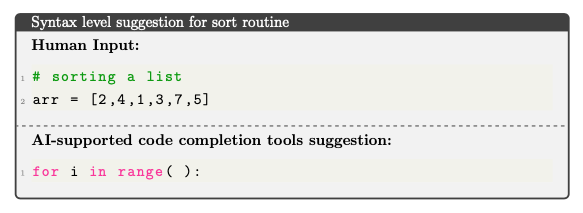
\includegraphics[width=\linewidth]{Figures/syntax.png}
    \caption{code suggestion of \cct{} at syntax level}
    \label{fig:syntax}
\end{figure}

The goal of this software abstraction level in our taxonomy is for a \cct{} to be able to suggest code without any syntactical errors.
The capabilities required by \cct{} to satisfy this level of abstraction are as follows:

\begin{enumerate}
    \item Suggested code should be syntactically correct.
    \item Suggested code should not produce any errors in code compilation.
\end{enumerate}

% \begin{tcolorbox}[title=Syntax level suggestion for sort routine,boxsep=.15mm]
%     %https://tex.stackexchange.com/questions/337909/tcolorbox-tcbline-style
% \textbf{Human Input:}
% \begin{lstlisting}[language={Python}]
% # sorting a list
% arr = [2,4,1,3,7,5]
% \end{lstlisting}
% \tcbline
% \textbf{\cct{} suggestion:}
% \begin{lstlisting}[language={Python}]
% for i in range( ):
% \end{lstlisting}
% \end{tcolorbox}
\subsection{Correctness}
\label{correctness}
Correctness is the second level of software abstraction in our taxonomy. 
\cct{} at this level should be capable of suggesting code that is not only syntactically correct but also solves the programming task. 
This level does not require \cct{} to suggest the best possible coding solution for the programming task but to be able to suggest a decent solution to the programming task which may or may not resolve all the edge cases of the given programming task.

For example, consider the programming task of performing a sorting operation on a list of numbers. To satisfy this level of abstraction, \cct{} should suggest a syntactically correct list sorting code, which is not required to be the most efficient way of sorting a list.
Figure~\ref{fig:correctness} shows the list sorting example and the Python code suggestion from \cct{} at this abstraction level, which performs the sorting operation.

\begin{figure}[hbt!]
    \centering
\begin{tcolorbox}[title=Correctness level suggestion for sort routine,boxsep=.15mm]
    %https://tex.stackexchange.com/questions/337909/tcolorbox-tcbline-style
\textbf{Human Input:}
\begin{lstlisting}[language={Python}]
# sorting a list
arr = [2,4,1,3,7,5]
\end{lstlisting}
\tcbline
\textbf{\cct{} suggestion:}
\begin{lstlisting}[language={Python}]
n = len(arr)
for i in range(n):
    for j in range(n-1):
        if arr[j] > arr[j+1]:
            temp = arr[j]
            arr[j] = arr[j+1]
            arr[j+1] = temp
print(arr)
\end{lstlisting}
\end{tcolorbox}
    \caption{Code suggestion of \cct{} at correctness level.}
    \label{fig:correctness}
\end{figure}

The goal of this software abstraction level in our taxonomy is for a \cct{} to be able to suggest a solution instead of the best one.
The capabilities required by \cct{} to satisfy this level of abstraction are as follows:

\begin{enumerate}
    \item Suggest a solution for a given programming task that may not be the optimal solution for that programming task.
    \item The solution suggested is not required to cover all the edge cases for that programming task.
    \item Satisfy requirements of all the levels below correctness in our taxonomy.
\end{enumerate}


\subsection{Paradigms and Idioms}
Paradigms and idioms are our taxonomy's third level of software abstraction. 
This level requires the code suggested by \cct{} to satisfy all the previous levels of abstractions and use common paradigms and language idioms in its code suggestions. 
These include common practices of solving a programming task. 

Returning to our running example of performing a sorting operation on a list of numbers. 
To satisfy this level of abstraction, \cct{} should suggest a syntactically correct list sorting code, using idiomatic ways in its code suggestions, like the Pythonic way of swapping items in a list~(line 5 in figure~\ref{fig:idioms}), As opposed to suggesting non-idiomatic approaches like creating another temporary variable to swap items in a list shown in correctness level~(figure~\ref{fig:correctness}).

Figure~\ref{fig:idioms} shows the sorting example and the Python code suggestions from \cct{} at this abstraction level.

\begin{figure}[hbt!]
    \centering
\begin{tcolorbox}[title=Idioms level suggestion for sort routine,boxsep=.15mm]
    %https://tex.stackexchange.com/questions/337909/tcolorbox-tcbline-style
\textbf{Human Input:}
\begin{lstlisting}[language={Python}]
# sorting a list
arr = [2,4,1,3,7,5]
\end{lstlisting}
\tcbline
\textbf{\cct{} suggestion:}
\begin{lstlisting}[language={Python}]
n = len(arr)
for i in range(n):
	for j in range(n-1):
		if arr[j] > arr[j+1]:
			arr[j], arr[j+1] = arr[j+1], arr[j]
print(arr)
\end{lstlisting}
\end{tcolorbox}
    \caption{Code suggestion of \cct{} at paradigms and idioms level.}
    \label{fig:idioms}
\end{figure}

The goal of this software abstraction level in the taxonomy is for \cct{} to detect and use commonly known idiomatic approaches and paradigms that occur in public code in its suggestions for suggesting code to solve a programming task.

The capabilities required by \cct{} to satisfy paradigms and idioms level of software abstraction are as follows:
\begin{enumerate}
    \item Identify common patterns like paradigms and language idioms in public code repositories~(training data).
    \item Use paradigms and language idioms in suggesting solutions for a programming task.
    \item Satisfy requirements of all the levels below paradigms and idioms in our taxonomy.
\end{enumerate}


\section{Design Smells}
Currently, Copilot does not support multi-file input, So it is not possible to evaluate its design suggestions, as software development process may include multiple folders with a file structure. 
Making Code completion tools adapt their suggestions to context specific issues such as variable naming conventions and formatting would be challenging as the existing guidelines are not standard in this space and mostly depend on context, The training dataset for AI driven development should also include rules such as idioms, best practices before tackling design level problems.
% Design smells or arch smells (Tushar Sharma)
\subsection{Design}
\label{design}
Design level is the top level of software abstraction in our taxonomy This level requires the suggested code suggest rational design practices in its code suggestions for a problem and satisfy all the previous levels of abstractions. Design practices are dependent on many factors like requirements, \cct{} should be capable of considering all the relevant factors before suggesting a design practice.

For example, considering the task of performing a sorting operation on a list of numbers. To satisfy this level of abstraction, \cct{} should suggest a syntactically correct list sorting code, using an algorithm which gives the best performance for that particular input scenario like suggesting quick sort algorithm~(avg time complexity = nlogn) instead of bubble sort algorithm~(avg time complexity = n\textsuperscript{2}).

The main goal of this level in the taxonomy is for a \cct{} to be able to pick algorithms and suggest design choices as per given scenario in its suggestions.
The capabilities required by a \cct{} to satisfy this level of abstraction are as follows
\begin{enumerate}
    \item Identify design and module level concerns in code files.
    \item Suggest design patterns and architectural tactics when prompted.
    \item Picking and suggesting the best applicable algorithm for a given scenario.
    \item Satisfy requirements of all previous levels of abstractions.
\end{enumerate}

% \begin{tcolorbox}[title=Code smells level suggestion for sort routine,boxsep=.15mm]
%     %https://tex.stackexchange.com/questions/337909/tcolorbox-tcbline-style
% \textbf{Human Input:}
% \begin{lstlisting}[language={Python}]
% # sorting a list
% arr = [2,4,1,3,7,5]
% \end{lstlisting}
% \tcbline
% \textbf{\cct{} suggestion:}
% \begin{lstlisting}[language={Python}, morekeywords={False, True}]
% swapped = False
% for i in range(len(arr)-1, 0, -1):
% 	for j in range(n):
% 		if arr[j] > arr[j+1]:
% 		    swapped = True
% 			arr[j], arr[j+1] = arr[j+1], arr[j]
% 	if not swapped:
% 	    break
% print(arr)
% \end{lstlisting}
% \end{tcolorbox}
\section{Chapter Summary}
In summary, we start this chapter by showing the methodology used in addressing \textbf{RQ-1.2} (How do \cct{} manage to suggest non-smelly code?). We first introduced the study setup with the input to Copilot and how it was restricted to deriving the best practice from the input and how the suggestions from Copilot were evaluated. We sampled best practices from AirBNB JavaScript coding style guide~\cite{airbnb_code}, and then compared it against Copilot suggestions. Based on results shown in Table~\ref{tab:all_bp}, Copilot struggles to suggest the best practices from widely used coding standards in its suggestions. 

In this chapter, we showed that Copilot struggles to detect and follow coding style guides  present in public repositories of GitHub and always suggest code that follows those coding style guides. The ideal behavior of \cct{} like Copilot in solving this problem is to detect the coding style guideline from existing code in the project and always suggest code that follows the guideline.

In the next chapter (chapter~\ref{chapter:framework}), we illustrate our taxonomy inspired from autonomous driving levels on the software abstraction hierarchy in \AISE{}, and delineate where \cct{} are currently best able to perform, and where more complex software engineering tasks overwhelm them.